\documentclass[../main.tex]{subfiles}

\begin{document}
\section{Simulation}\label{sec:results0}
\subsection{Numerical setup}\label{sec:numerical}
The 2D incompressible Navier-Stokes equations are forced in a periodic domain of size $2\pi \times 2\pi$ with a forcing term that is located in a disk of radius $\pi/k_r$ centered at the origin.  The range of values for the parameter $k_r$ is taken to be $\{8, 16, 32, 64\}$ and in all the cases the size of the vortices, which is controlled by $k_\ell$, is set to $k_\ell = 4 k_r$. The parameter $k_r$ being one of those values in the previous set represents how smaller the perturbation region is (in diameter) compared to the domain size ($2\pi$). The other parameter $k_\ell$ accounts for the size of the vortices, as $1/k_\ell$ gives a typical length scale of the vortices.~\cref{fig:forcing} shows a graphical representation of the forcing term for two different values of $k_r$.
\begin{figure}[ht]
	\centering
	\begin{subfigure}{0.44\textwidth}
		\centering
		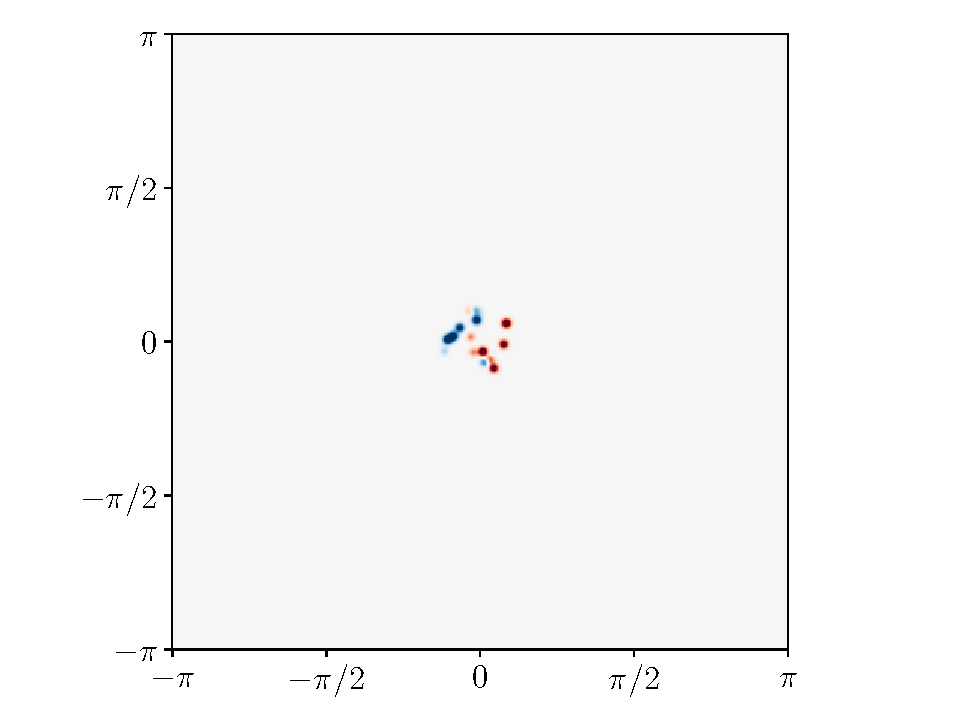
\includegraphics[width=\textwidth]{images/forcing32_8.pdf}
		\caption{$k_r = 8$}
	\end{subfigure}\hspace{0.04\textwidth}
	\begin{subfigure}{0.44\textwidth}
		\centering
		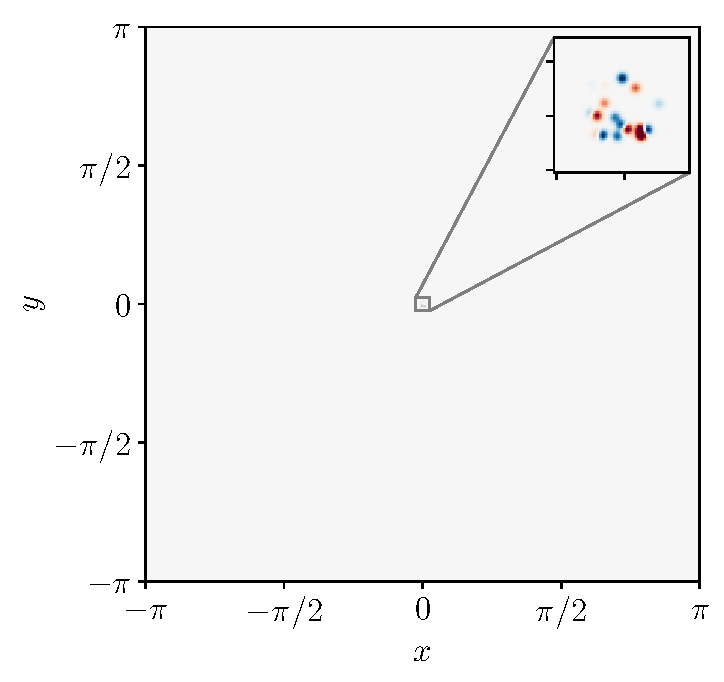
\includegraphics[width=\textwidth]{images/forcing32_64.pdf}
		\caption{$k_r = 64$}
	\end{subfigure}
	\caption{Vorticity forcing term for different values of $k_r$. Red colors and blue colors mean different direction of rotation for each vortex. The reader may notice that indeed in the first plot the diameter of the forcing region is about 8 times smaller than the total size of the domain. In the second plot, this property is less noticeable, but it is still true, this case being 64 times smaller.}\label{fig:forcing}
\end{figure}

The Reynolds number is the other parameter that plays an important role in the whole simulation. This project has simulated fluid flows for Reynolds numbers within the set $\{0.25, 0.5, 1, 2, 4, 8, 16, 32, 64, 128\}$, each of those requiring different resolution as the Reynolds number is increased in order to capture the smallest scales where energy gets dissipated by viscosity.

A pseudo-spectral method is used to solve the Navier-Stokes equations, based on the Fourier basis and then using an improved 2nd-order low-storage Runge-Kutta method to integrate the resulting ordinary differential equation. As explained in~\cite{rungekutta}, this method differs from the conventional Runge-Kutta methods by reducing the amount of storage needed for each iteration at the expense of roughly doubling the time needed for evaluating the temporal derivatives at the same order as the usual Runge-Kutta methods. Specifically, if $\vf{\widehat{\psi}}_n$ is the vector containing all the coordinates at the $n$-th step of the integration, the scheme follows the subsequent steps:
\begin{enumerate}
	\item Copy $\vf{\widehat\psi}_n$ into $\vf{\widehat\psi}_*$.
	\item For $i = s, \ldots, 1$, $s$ being the number of stages of the Runge-Kutta method, update $\vf{\widehat\psi}_*$ as follows:
	      \begin{equation}
		      \vf{\widehat\psi}_* \leftarrow \vf{\widehat\psi}_n + \Delta t \frac{\vf{F}(\vf{\widehat\psi}_*)}{i}
	      \end{equation}
	      where $\vf{F}$ represents the field that defines the differential equation for ${\widehat\psi}$.
	\item Set $\vf{\widehat\psi}_{n+1} := \vf{\widehat\psi}_*$.
\end{enumerate}
In the second step, the evaluation of $\vf{F}$ is done in an explicit-exact manner. This means that the non-linear term is treated explicitly in time, while the linear terms are solved exactly using their exponential solution. For more information about the scheme, the reader is encouraged to read the article from~\cite{rungekutta} or check the source codes in the link provided below. In this work, $s=4$ is used for all simulations. While this produces a formal order of accuracy of 2, the errors are generally smaller compared to those of a standard second-order Runge-Kutta method.

The codes are run in two supercomputer centers, IDRIS\footnote{For more information about the resources they provide, check their website: \url{http://www.idris.fr/} (accessed on June 30, 2024).} and MESOPSL\footnote{For more information about the resources they provide, check their website: \url{https://wwwmesopsl-new.obspm.fr/} (accessed on June 30, 2024).}, using 40 to 80 cores, depending on the simulation. Two different kinds of simulations are performed: (fully) parallel simulations and embarrassingly parallel simulations. In the parallel simulations, the Fourier domain is divided among all the processors, allowing them to work simultaneously on different parts of the problem. In the embarrassingly parallel simulations, each simulation runs independently on a single core. Multiple simulations are executed concurrently, one on each available core, and the results are averaged afterwards to obtain more accurate conclusions. This project uses MPI compilers to do the parallelism. Details about the parallelization of the code will not be delved into, but the main idea will be explained.

They key piece of the parallelization of any pseudo-spectral method is the efficient computation of the multidimensional Fourier transform. As a starting point, one of the dimensions of the physical domain, of size $N\times N$, is split, creating several subdomains of sizes $\tilde{N}\times N$, where $\tilde{N} \simeq N/N_\mathrm{cores}$ and $N_\mathrm{cores}$ is the number of cores used. Each core is responsible for computing $\tilde{N}$ 1D real-to-complex Fourier transforms using the standard Fast Fourier Transform (FFT) algorithm which reduces the operations from $\mathcal{O}(N^2)$, using the naive approach, to $\mathcal{O}(N\log N)$. Since the initial data is real-valued, the complex-valued transformed data is then stored in an array $\tilde{N}\times (N/2 + 1)$, which is enough to store all the necessary information. Next, MPI communication is carried out in order to gather all the data, transpose it, and then split it again to produce slices of size $\bar{N}\times N$, where $\bar{N} \simeq (N/2 + 1)/N_\mathrm{cores}$. Each core is, similarly as before, responsible for computing $\bar{N}$ 1D complex-to-complex Fourier transforms. Finally, all the data is gathered again to produce the desired FFT resulting in a memory block of size $(N/2 + 1)\times N$ consisting of complex-valued numbers. If the reader is interested in the details, the article from~\cite{mpi} is highly recommended.

For the parallel code, a variable time step is used throughout the whole simulations in order to take into account the advection stability condition. For the embarrassingly parallel code, a fixed time step is used, for the purpose of better comparing the results between the different runs from the same simulation. The time step is chosen by eye after studying the evolution of the time steps during the variable-time-step fully parallel simulations.~\cref{tab:simulations} shows the different simulations performed during the project as well as the resolution in physical space used in each case.
\begin{table}[ht]
	\centering
	\def\tickgreen{\textcolor{color_green3}{\ding{51}}}
	\def\tickblue{\textcolor{color_blue3}{\ding{51}}}
	% set space between columns
	\setlength{\tabcolsep}{5pt}
	% set space between rows
	\renewcommand{\arraystretch}{1.5}
	\begin{tabular}{c|cccccccccc}
		\diagbox[width=\dimexpr \textwidth/16+2\tabcolsep\relax, height=1cm]{$k_r$}{$\Re$} & 0.25               & 0.5                & 1                  & 2                           & 4                            & 8                            & 16                           & 32                           & 64                  & 128                 \\\hline
		8                                                                                  & \tickgreen$_{512}$ & \tickgreen$_{512}$ & \tickgreen$_{512}$ & \tickgreen\tickblue$_{512}$ & \tickgreen\tickblue$_{1024}$ & \tickgreen\tickblue$_{1024}$ & \tickgreen\tickblue$_{1024}$ & \tickgreen\tickblue$_{2048}$ & \tickgreen$_{2048}$ & \tickgreen$_{4096}$ \\
		16                                                                                 &                    &                    &                    & \tickblue$_{1024}$          & \tickblue$_{2048}$           & \tickgreen\tickblue$_{2048}$ & \tickgreen\tickblue$_{2048}$ & \tickgreen\tickblue$_{2048}$ & \tickgreen$_{4096}$ & \tickgreen$_{4096}$ \\
		32                                                                                 &                    &                    &                    & \tickblue$_{2048}$          & \tickblue$_{4096}$           & \tickgreen\tickblue$_{4096}$ & \tickgreen\tickblue$_{4096}$ & \tickgreen\tickblue$_{4096}$ & \tickgreen$_{8192}$ & \tickgreen$_{8192}$ \\
		64                                                                                 &                    &                    &                    &                             &                              & \tickgreen$_{8192}$          & \tickgreen$_{8192}$          & \tickgreen$_{8192}$          &                     &                     \\
	\end{tabular}
	\caption{Simulations carried out during the study varying the Reynolds number and the forcing parameter $k_r$. In all cases $k_\ell$ is taken as $k_\ell = 4k_r$. The green checkmark symbols indicate the simulations executed in parallel, splitting the domain between different cores. The blue checkmark symbols indicate the simulations conducted in an embarrassingly parallel manner, where each simulation runs independently across multiple cores simultaneously to generate statistical results. In each cell, the number indicates the resolution in each dimension employed, which have been proved (a posteriori) to be enough to well-resolve the system.}\label{tab:simulations}
\end{table}

The reader may observe that the resolution increases as both the Reynolds number and the forcing parameter $k_r$ increase. For the former, the resolution is increased to resolve the smaller scales that appear in the system, which play an essential role in dissipating energy through viscosity. Thus, as $\Re$ increases, $\nu$ decreases, and the predicted Kolmogorov wave number, where dissipation occurs, becomes larger. For the latter, the resolution is increased as the wave numbers of the forcing region rise, thereby shifting the energy injection to higher frequencies. It is worth-noting that the resolution in Fourier space is not the same as the one in physical space. Specifically, as mentioned before, the Fourier resolution is one third of the physical resolution in each dimension. This adjustment is made to avoid common aliasing errors that may arise when computing non-linear terms in Fourier space. Concerning the total time of integration, the simulations were stopped when enough vortices had reached the boundaries of the domain, which was determined by eye.

The system of differential equations modeling the point vortex dynamics (see \cref{eq:pointvortexA_soft,eq:pointvortexB_soft}) is integrated using a Runge-Kutta (7)8 method with adaptive time-stepping based on the Fehlberg error estimate. Briefly, these adaptative Runge-Kutta methods are based on the idea of using two different approximations of the solution at each step, in this case, one of order 7 and another of order 8. Then, the difference between both approximations is used to estimate the error between one of the approximations and the real solution. If the error is below a certain threshold, the time step is increased, and if it is above it, the time step is decreased. The simulations for the point vortex model are conducted, as opposed to the integration of the Navier-Stokes equations, in a personal computer and in a single core. In this latter simulation there is only one parameter to control, which is the radius of the perturbation region, $k_r$. As the simulation is less computationally expensive, the range of values for $k_r$ is increased to $\{8, 16, 32, 64, 128, 256\}$ compared to the Navier-Stokes simulations.

\newcommand{\theoldfootnote}{\thefootnote}
\renewcommand{\thefootnote}{\fnsymbol{footnote}}
All the codes and data used for the simulations as well as animations of the dynamics of both problems are available in the following repository: \url{https://github.com/victorballester7/final-master-thesis} (accessed on June 26, 2024). The pseudo-spectral codes on that repository are based on previous works from Pablo Mininni\footnote[3]{Professor in the Department of Physics at the University of Buenos Aires. Webpage: \url{http://wp.df.uba.ar/mininni/} (accessed on June 25, 2024).} and Alexandros Alexakis. The repository of Pablo Mininni is available at \url{https://github.com/pmininni/GHOST} (accessed on June 25, 2024).
\renewcommand{\thefootnote}{\theoldfootnote}
\subsection{Results}\label{sec:results}
The results of the simulations are presented in this section. The first part is devoted to the results of the Navier-Stokes simulations, while the second part is dedicated to the results of the point vortex simulations.

We start showing how the vortices spread across the domain in a visual manner.
\begin{figure}[ht]
	\centering
	\begin{subfigure}{0.44\textwidth}
		\centering
		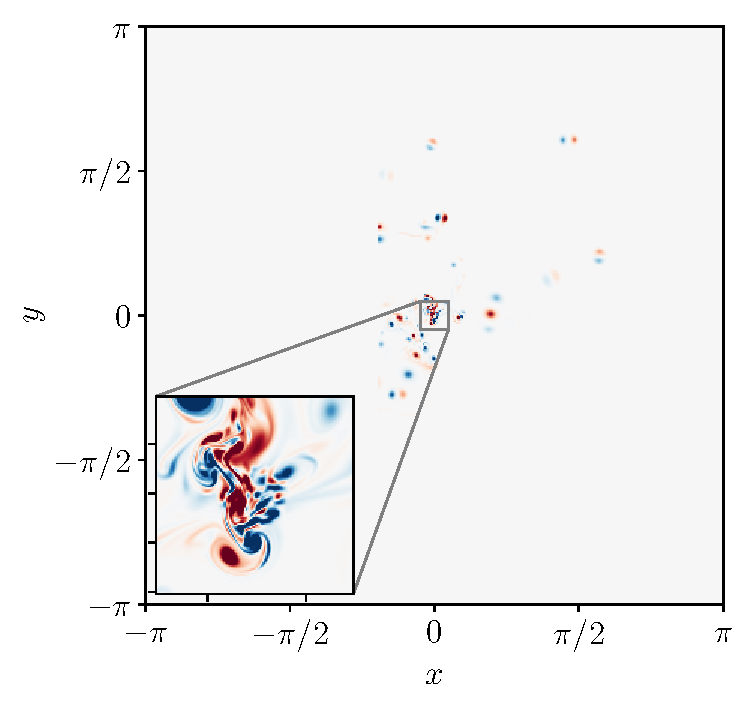
\includegraphics[width=\textwidth]{images/domainRe32kdn64.pdf}
		\caption{$k_r = 64$, $\Re = 32$}
	\end{subfigure}\hspace{0.04\textwidth}
	\begin{subfigure}{0.44\textwidth}
		\centering
		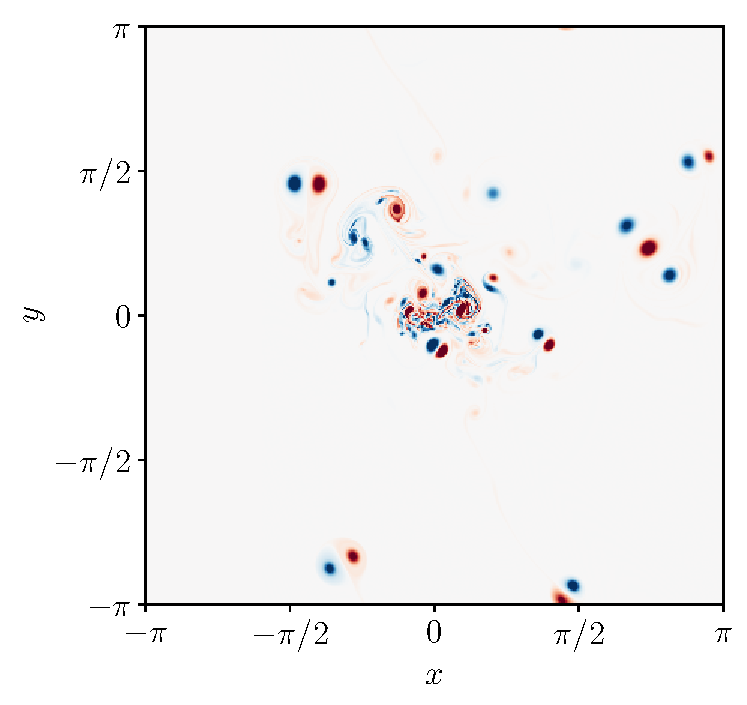
\includegraphics[width=\textwidth]{images/domainRe128kdn16.pdf}
		\caption{$k_r = 16$, $\Re = 128$}
	\end{subfigure}
	\caption{Vorticity plots for different values of $k_r$ and $\Re$. The left-hand side figure is integrated with a resolution of $8192\times 8192$ and the right figure is integrated with a resolution of $4096\times 4096$.}\label{fig:vortices_evo}
\end{figure}

\cref{fig:vortices_evo} shows the vorticity plot at two different time slices for the driven Navier-Stokes equation. The most notable feature is that the vortices appear more intense in the plot on the right compared to the plot on the left. This can be attributed to two main reasons. Firstly, the Reynolds number is smaller in the left-hand-side plot, causing dissipation by viscosity to have a more significant impact, leading to a quicker decay of the intensity of the vortices. Secondly, the initial size of the vortices in the plot on the left is four times smaller than in the plot on the right, which restricts their growth in size as time progresses.
\begin{figure}[!ht]
	\centering
	\begin{subfigure}{0.44\textwidth}
		\centering
		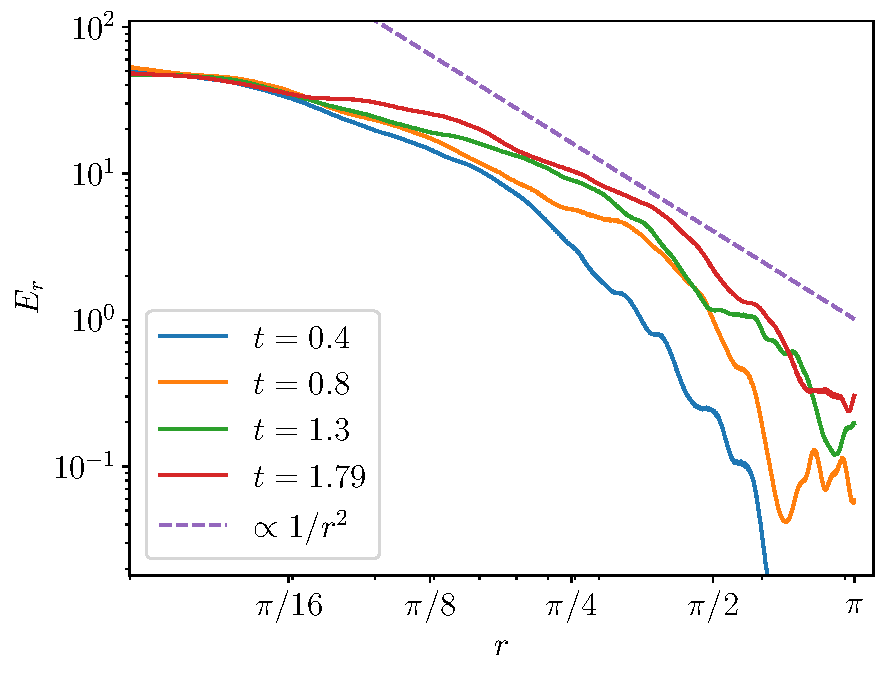
\includegraphics[width=\textwidth]{images/Energy_t.kdn16.test6.pdf}
		\caption{$k_r = 16$, $\Re = 16$}
	\end{subfigure}\hspace{0.04\textwidth}
	\begin{subfigure}{0.44\textwidth}
		\centering
		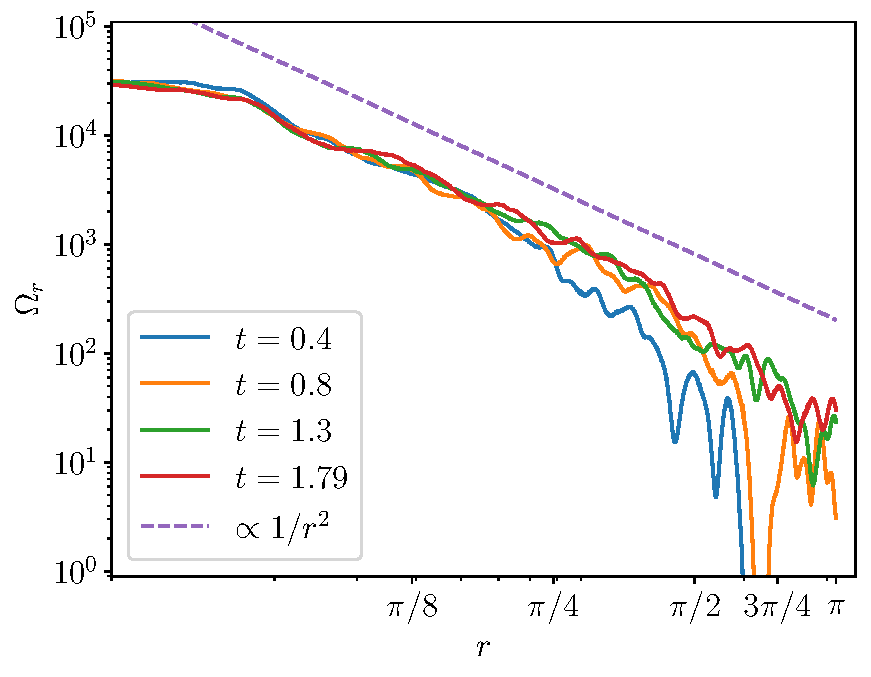
\includegraphics[width=\textwidth]{images/Enstrophy_t.kdn16.test6.pdf}
		\caption{$k_r = 16$, $\Re = 16$}
	\end{subfigure}\\[0.5cm]
	\begin{subfigure}{0.44\textwidth}
		\centering
		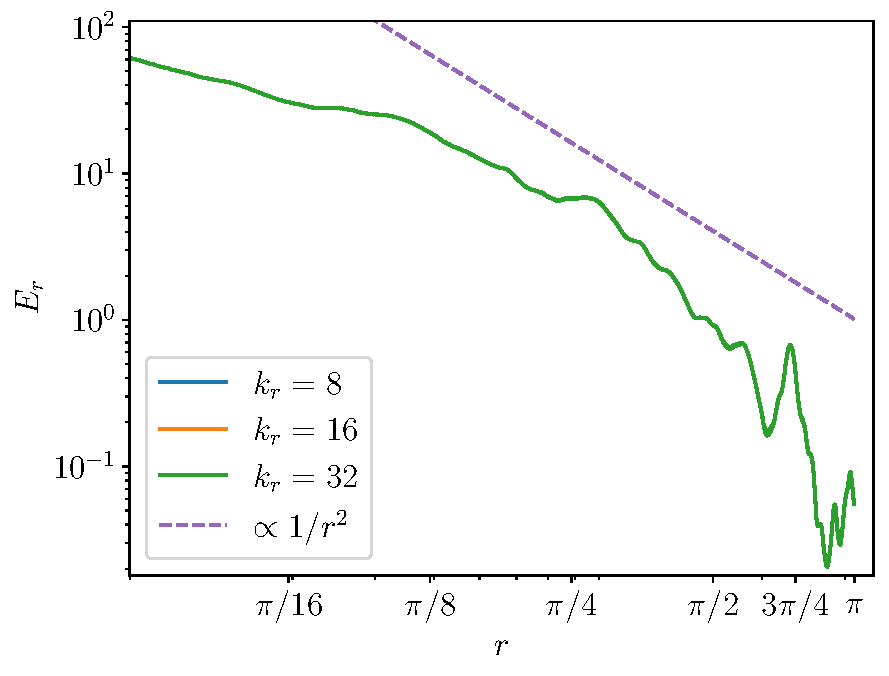
\includegraphics[width=\textwidth]{images/Energy_kdn.test7.059.pdf}
		\caption{$\Re = 32$}
	\end{subfigure}\hspace{0.04\textwidth}
	\begin{subfigure}{0.44\textwidth}
		\centering
		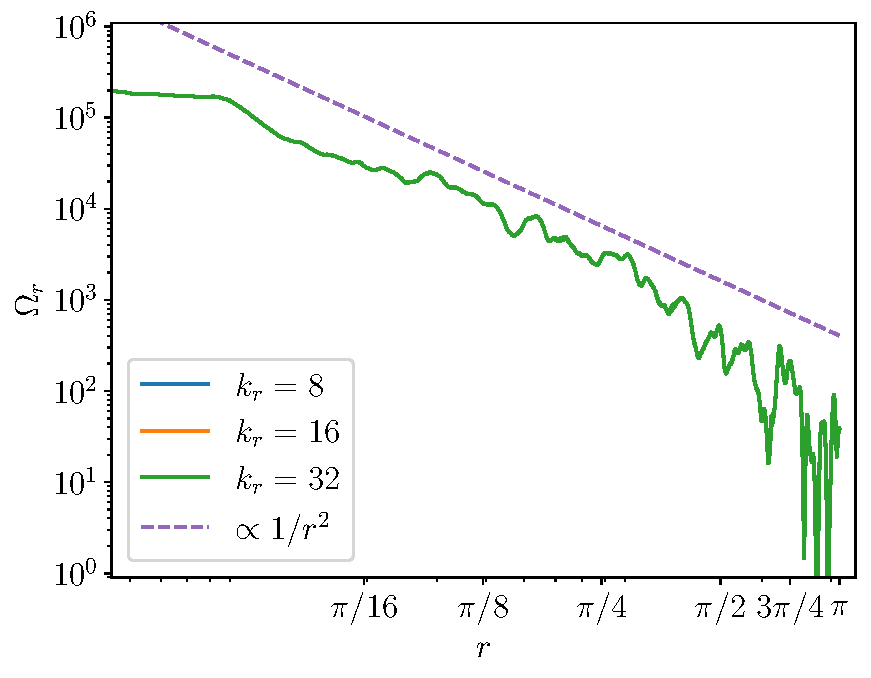
\includegraphics[width=\textwidth]{images/Enstrophy_kdn.test7.059.pdf}
		\caption{$\Re = 32$}
	\end{subfigure}\\[0.5cm]
	\begin{subfigure}{0.44\textwidth}
		\centering
		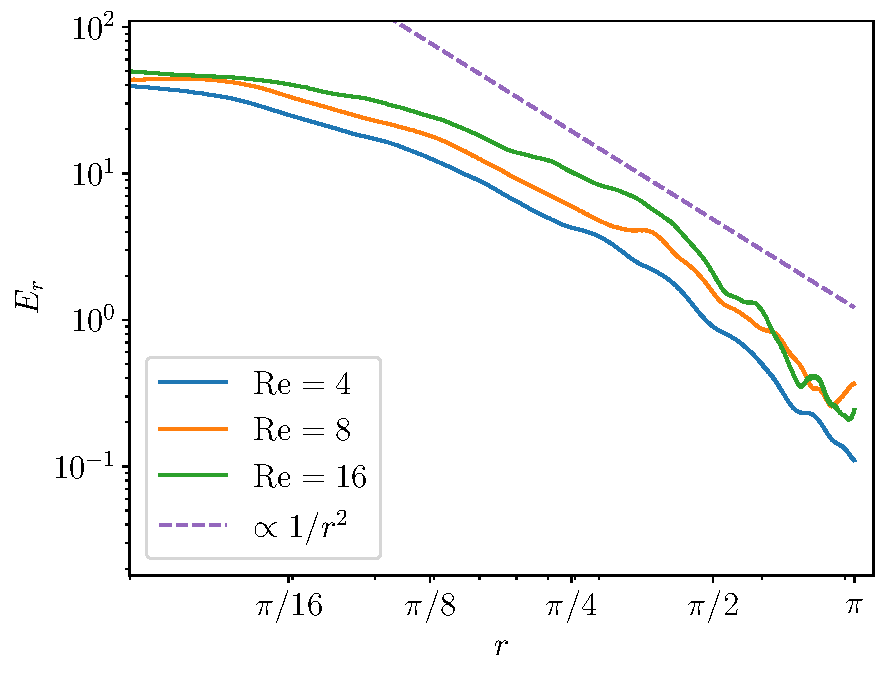
\includegraphics[width=\textwidth]{images/Energy_Re.kdn16.175.pdf}
		\caption{$k_r = 16$}
	\end{subfigure}\hspace{0.04\textwidth}
	\begin{subfigure}{0.44\textwidth}
		\centering
		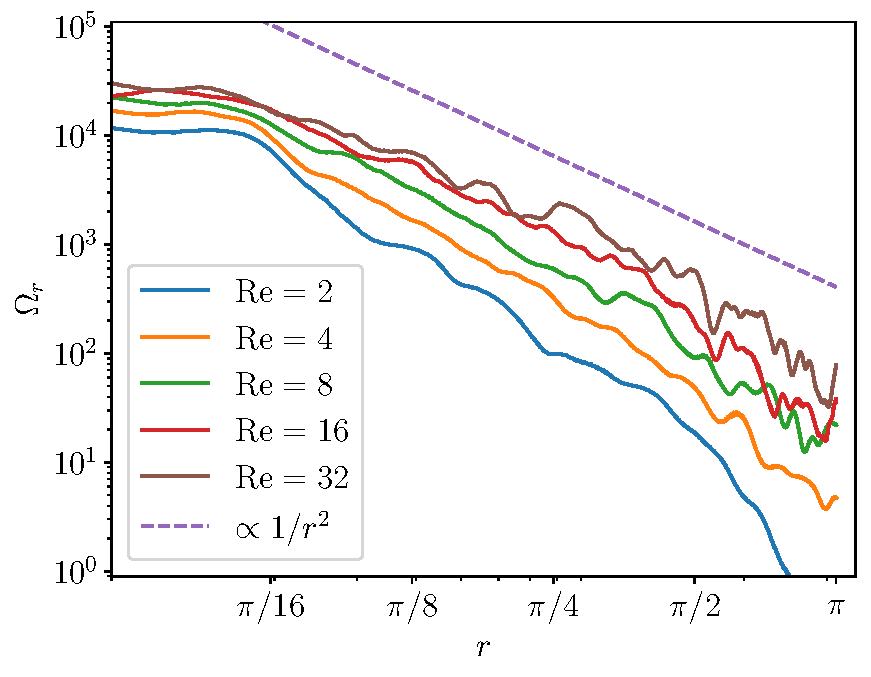
\includegraphics[width=\textwidth]{images/Enstrophy_Re.kdn16.175.pdf}
		\caption{$k_r = 16$}
	\end{subfigure}
	\caption{Energy and enstrophy profiles for different values of time, $k_r$ and $\Re$. The left-hand side figures show the respective plots for the energy while in the right-hand side, the enstrophy profiles are displayed. The top plots show the profiles for different slices of time for a fixed $k_r=16$ and $\Re=16$. The units of time are those determined from the Reynolds number, that is $k_\ell^{-4/3}/\epsilon^{1/3}$, where $\epsilon$ is given in \cref{eq:epsilon}. The middle plots show the profiles for several radius of the perturbation region at fixed time $t=1.66$ and fixed $\Re=32$. The bottom plots show the profiles for different Reynolds numbers at fixed time $t=1.75$ and fixed $k_r=16$. In all the plots the dashed line represents a function of the form $f(r)=A/r^2$ with $A$ being a constant.}\label{fig:energy_enstrophy}
\end{figure}

With this glimpse into the dynamics of the system, we now proceed to analyze the energy and enstrophy distributions. The following set of plots in \cref{fig:energy_enstrophy} show the energy and enstrophy evolution as a function of the distance to the center of the forcing disk in three different categories: firstly, a Reynolds number and a parameter $k_r$ are picked and the distributions of energy and enstrophy are plotted for different times; secondly, plots varying $k_r$ at fixed time $t=1.66$ and for $\Re=32$ are shown, and finally, the energy and enstrophy profiles for different Reynolds numbers at fixed time $t=1.75$ and $k_r=16$ are displayed. All the data is obtained by averaging the results of 48 simulations, each one with a different random seed, using embarrassingly parallel simulations.

The first feature that the reader may extract from all the plots is that generally the power laws that the quantities appear to follow are more clear and consistent in the vorticity plots, rather than in the energy ones. This, together with the fact that the vorticity plots are more spiky and the energy plots smoother, may be attributed to the fact that vorticity is a quantity more localized than energy, taking only high values where the vortices are located (see \cref{fig:vortices_evo}). On the other hand, the energy is more widely distributed across the domain because it is proportional to the square of the velocity, unlike vorticity, which depends on the rotation of the fluid. In a sense, this implies that there is more data available for averaging the energy than for the enstrophy, hence the smoother profiles in the energy plots.

On the top two plots of \cref{fig:energy_enstrophy}, an increase of energy to outer rings of the domain is observed as time increases, which starts answering one of the initial questions posed in the introduction about whether the energy would remain localized around the perturbation region. In the analogous vorticity plot at larger rings, more variance is observed in the curves for $t=0.4$ and $t=0.8$, compared to the curves for $t=1.3$ and $t=1.79$. This is attributed to the fact that in some simulations, only a few vortices manage to reach those outer layers of the domain at early times, unlike at later times when most simulations already contain many vortices in those outer layers.

The middle plots show the same evolution of the profiles of energy and enstrophy as a function of the radius of the annuli inside the domain. The most noticeable characteristic on the vorticity plot is that the supposed power law extends to smaller radii as $k_r$ increases. This is expected, as a larger $k_r$ is equivalent to decreasing the size of the forcing region, thereby shifting the observed features associated with smaller $k_r$ to different spatial locations, earlier in space. Moreover, before the power law is reached, the vorticity profiles show a roughly constant profile, which indicates the presence of a region where the vortices are equally distributed, i.e.\ the perturbation region. Indeed, the reader may observe that this roughly constant part of each curve finishes for $k_r=8$ at $\simeq \pi/8$, for $k_r=16$ at $\simeq \pi/16$ and for $k_r=32$ at $\simeq \pi/32$. With the energy profiles, a similar but less pronounced behavior is observed, which aligns with the previous argument regarding the smoothness of the energy profiles.

Finally, the bottom plots show, at fixed $k_r$ and fixed time, energy and enstrophy profiles for several Reynolds numbers. The remarkable feature here is that an increase in magnitude of both quantities is seen as the Reynolds number increases. This is expected, as viscosity in lower Reynolds numbers plays a more important role in dissipating energy, thereby stabilizing the dynamics of the system. The reader may also observe the constant behavior of the profiles for the range of $r\in [0,\pi/16]$ in the vorticity plots, which is consistent with the previous observations.

Next, the quantities $\mathcal{R}_E$ and $\mathcal{R}_\Omega$ are computed for the Navier-Stokes simulations and their evolution in time is plotted in \cref{fig:energy_enstrophy_mean} for several values of the Reynolds number and fixing the size of the perturbation region to $k_r=16$.
\begin{figure}[ht]
	\centering
	\begin{subfigure}{0.44\textwidth}
		\centering
		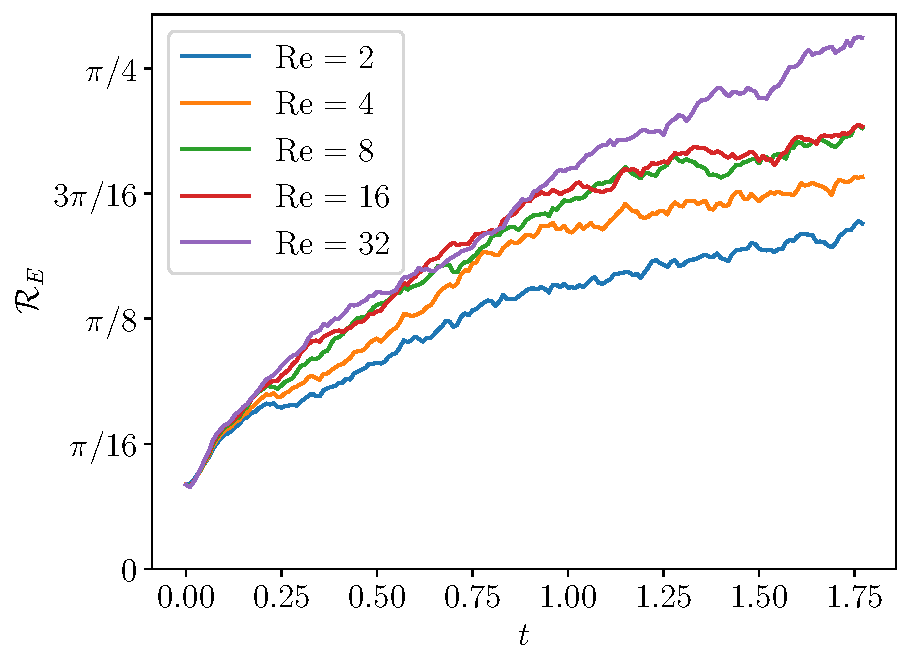
\includegraphics[width=\textwidth]{images/EnergyMeanRadius_Re.kdn16.pdf}
		\caption{Energy mean radius}
	\end{subfigure}\hspace{0.04\textwidth}
	\begin{subfigure}{0.44\textwidth}
		\centering
		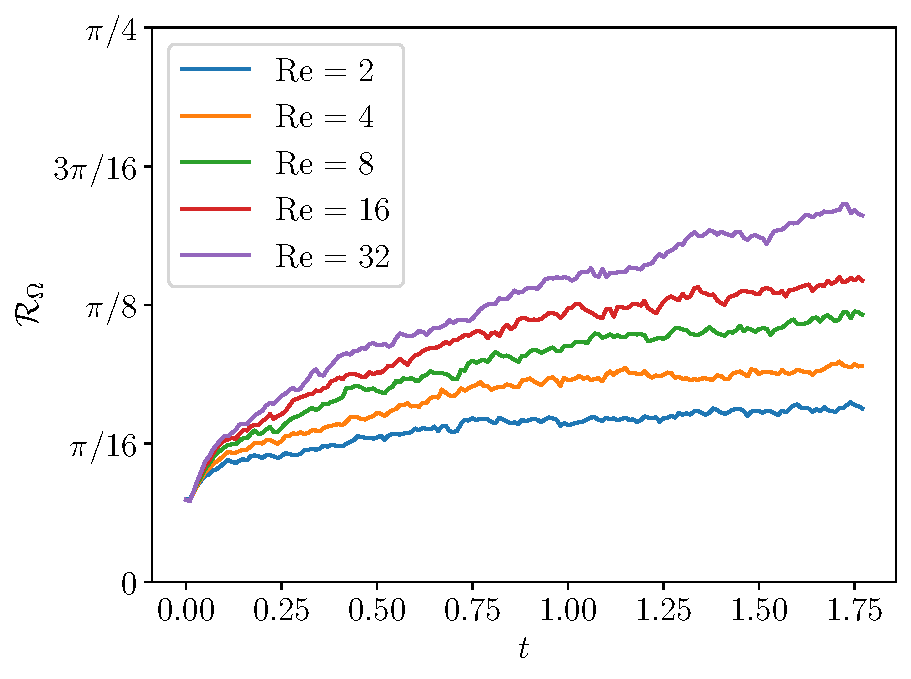
\includegraphics[width=\textwidth]{images/EnstrophyMeanRadius_Re.kdn16.pdf}
		\caption{Enstrophy mean radius}\label{fig:enstrophy_mean}
	\end{subfigure}
	\caption{Mean energy radius and mean enstrophy radius for several runs varying the Reynolds number at fixed $k_r=16$.}\label{fig:energy_enstrophy_mean}
\end{figure}

In all cases it is observed an increasing tendency, although the rate changes in time and also in the Reynolds number. Specifically in the enstrophy plot a separation between the different plots can be clearly seen, but the range of $\mathcal{R}_\Omega$ is smaller than the one of $\mathcal{R}_E$, likely due to the localizing nature of the vorticity. Based on this data, it is plausible to conclude that no matter how small the forcing region is, energy spreads throughout the entire domain given enough time, provided that viscosity is sufficiently low to allow vortices to persist without dissipating. It is understood that in order to properly and securely claim this statement, the simulations should have been run for longer times and higher Reynolds numbers.

The second part of this section is reserved to the results of the point vortex simulations. Here vortices are input at a constant rate in the center of the domain and they are removed whenever they reach the boundary of the box. Vortices are defined in terms of their circulation which is assumed to follow a standard normal distribution for all vortices.~\cref{fig:pointvortices} shows two different simulations changing the radius of the perturbation region. The plot on the right shows a higher density of vortices than the plot on the left, but as \cref{fig:numvortices} indicates, the density distribution is similar in both cases. In the first case, the stationary state is reached with a total number of around $ 400$ vortices inside the domain, while in the case for $k_r=128$ the total number of vortices is roughly $3300$.
\begin{figure}[ht]
	\centering
	\begin{subfigure}{0.44\textwidth}
		\centering
		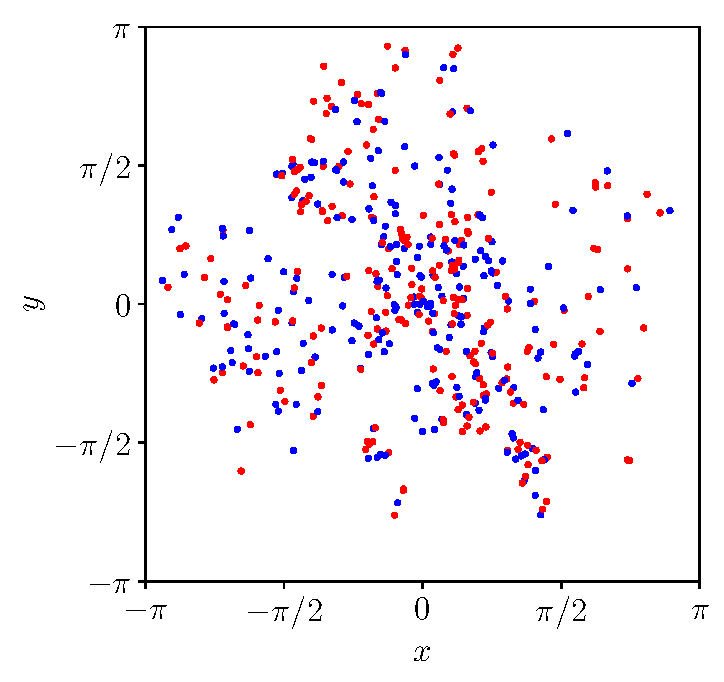
\includegraphics[width=\textwidth]{images/pointvortices.R4.00440.pdf}
		\caption{$k_r = 16$}
	\end{subfigure}\hspace{0.04\textwidth}
	\begin{subfigure}{0.44\textwidth}
		\centering
		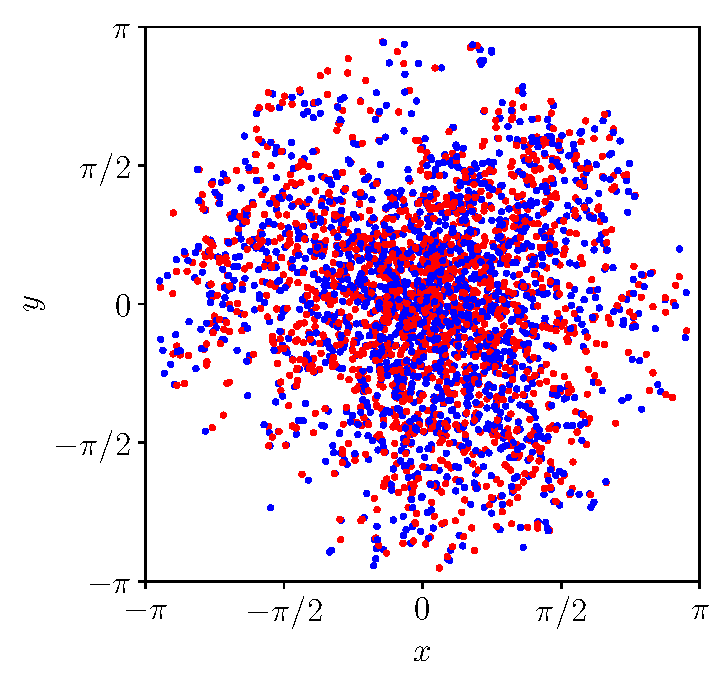
\includegraphics[width=\textwidth]{images/pointvortices.R32.00550.pdf}
		\caption{$k_r = 128$}
	\end{subfigure}
	\caption{Evolution of the point vortex simulation for different sizes of the perturbation region. Red colors and blue colors mean different direction of rotation for each vortex.}\label{fig:pointvortices}
\end{figure}

We conclude this section by analyzing certain properties of the point vortex model to compare them with the Navier-Stokes simulations. First, \cref{fig:numvortices} represents the density profile of the number of vortices as a function of the distance to the center of the box. This density is a linear density, by means that it is defined as the number of vortices in a thin annulus inside the domain divided by the radius of the annulus. The curves for different sizes of the forcing region are shown in that plot. The reader may observe that all the curves follow a similar behavior. A note should be done at this point. Unlike the other curves, the curve corresponding to the region with $k_r=256$ is slightly below the others. This discrepancy arises because the stationary state for that simulation had not yet been reached by the end of the run. Despite this, the curve remains consistent with the others. The reader may also observe a interesting power law $\propto 1/r$ which fits reasonably well in the middle region of the range of $r$. This in turn implies a constant flux of vortices in that subregion.

\cref{fig:numvortices_meanradius} shows a mean radius weighted with the number of vortices as a function of time, according to its definition in \cref{eq:meanradius_vortices}. This simulation differs from the others in the point vortex problem in that no vortices are removed at any time, making the integration domain the entire $\RR^2$. This is done to avoid the appearance of a stationary state in the system. As a first observation, the reader observes a growing behavior which resembles, in the middle stages, to the behavior of the enstrophy mean radius in the Navier-Stokes simulations (see \cref{fig:enstrophy_mean}). It has been proved that the curve is well fitted with the law $A\sqrt{t}$, except for the very early times. As time increases and vortices evolve to the outer regions of the domain, the curve starts to differ from the ones observe in the Navier-Stokes simulations. This may be attributed to the effect of the boundary conditions. In the Navier-Stokes simulations, the boundary conditions are periodic, thus allowing the vortices to travel \emph{backwards} towards the center of the domain. In the point vortex simulations, the domain is open and the tendency of pairs of vortices to travel in an almost straight line, due to its similar magnitude of circulation, is not blocked.

\begin{figure}[ht]
	\centering
	\begin{minipage}[t]{0.44\textwidth}
		\centering
		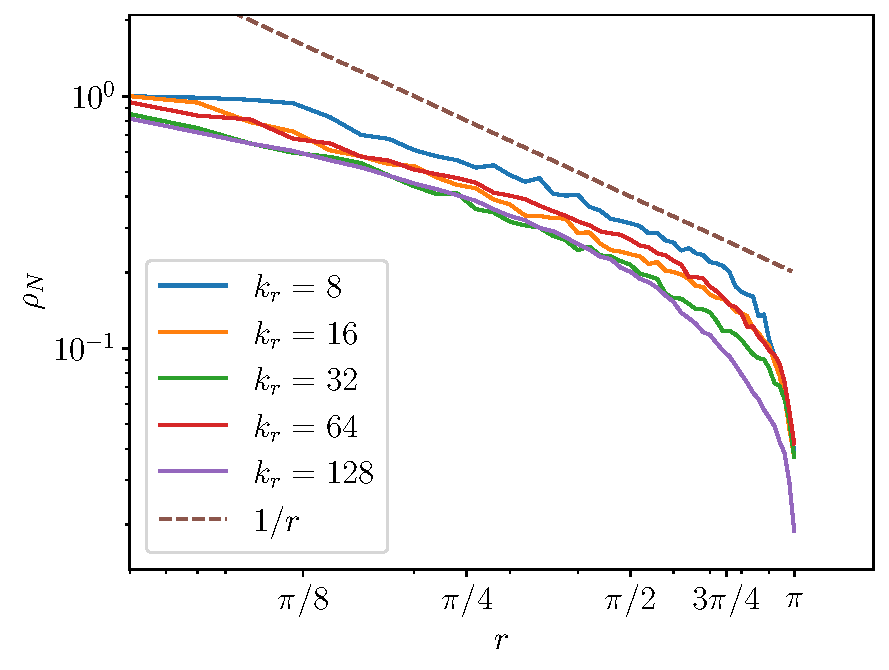
\includegraphics[width=\textwidth]{images/NumVortices.pdf}
		\caption{Density profile of the number of vortices as a function of the distance to the center of the perturbation region. The curves are averaged once a stationary state is reached and then they are normalized by their maximum value which is attained near the forcing region.
		}\label{fig:numvortices}
	\end{minipage}\hspace{0.04\textwidth}
	\begin{minipage}[t]{0.44\textwidth}
		\centering
		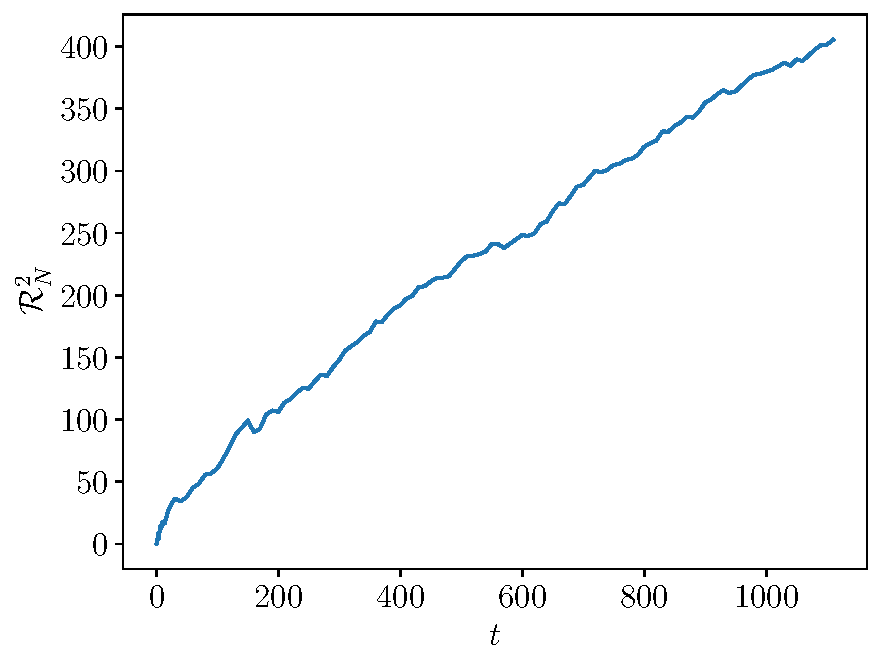
\includegraphics[width=\textwidth]{images/NumVorticesMeanRadius.pdf}
		\caption{Mean radius weighted with the number of vortices (following the definition in \cref{eq:meanradius_vortices}) as a function of time. The units of time are those determined from the circulation $\Gamma$ of the vortices and the natural length-scale $k_r^{-1}$, giving $1/(\Gamma k_r^2)$.}\label{fig:numvortices_meanradius}
	\end{minipage}
\end{figure}

\end{document}
